%!TeX encoding = UTF-8
%!TeX program = xelatex
\documentclass[notheorems, aspectratio=54]{beamer}
% aspectratio: 1610, 149, 54, 43(default), 32

\usepackage{latexsym}
\usepackage{amsmath,amssymb}
\usepackage{mathtools}
\usepackage{color,xcolor}
\usepackage{graphicx}
\usepackage{algorithm}
\usepackage{amsthm}
\usepackage{lmodern} % 解决 font warning
% \usepackage[UTF8]{ctex}
\usepackage{animate} % insert gif

\usepackage{lipsum} % To generate test text 
\usepackage{ulem} % 下划线,波浪线

\usepackage{listings} % display code on slides; don't forget [fragile] option after \begin{frame}

% ----------------------------------------------
% tikx
\usepackage{framed}
\usepackage{tikz}
\usepackage{pgf}
\usetikzlibrary{calc,trees,positioning,arrows,chains,shapes.geometric,%
    decorations.pathreplacing,decorations.pathmorphing,shapes,%
    matrix,shapes.symbols}
\pgfmathsetseed{1} % To have predictable results
% Define a background layer, in which the parchment shape is drawn
\pgfdeclarelayer{background}
\pgfsetlayers{background,main}

% define styles for the normal border and the torn border
\tikzset{
  normal border/.style={orange!30!black!10, decorate, 
     decoration={random steps, segment length=2.5cm, amplitude=.7mm}},
  torn border/.style={orange!30!black!5, decorate, 
     decoration={random steps, segment length=.5cm, amplitude=1.7mm}}}

% Macro to draw the shape behind the text, when it fits completly in the
% page
\def\parchmentframe#1{
\tikz{
  \node[inner sep=2em] (A) {#1};  % Draw the text of the node
  \begin{pgfonlayer}{background}  % Draw the shape behind
  \fill[normal border] 
        (A.south east) -- (A.south west) -- 
        (A.north west) -- (A.north east) -- cycle;
  \end{pgfonlayer}}}

% Macro to draw the shape, when the text will continue in next page
\def\parchmentframetop#1{
\tikz{
  \node[inner sep=2em] (A) {#1};    % Draw the text of the node
  \begin{pgfonlayer}{background}    
  \fill[normal border]              % Draw the ``complete shape'' behind
        (A.south east) -- (A.south west) -- 
        (A.north west) -- (A.north east) -- cycle;
  \fill[torn border]                % Add the torn lower border
        ($(A.south east)-(0,.2)$) -- ($(A.south west)-(0,.2)$) -- 
        ($(A.south west)+(0,.2)$) -- ($(A.south east)+(0,.2)$) -- cycle;
  \end{pgfonlayer}}}

% Macro to draw the shape, when the text continues from previous page
\def\parchmentframebottom#1{
\tikz{
  \node[inner sep=2em] (A) {#1};   % Draw the text of the node
  \begin{pgfonlayer}{background}   
  \fill[normal border]             % Draw the ``complete shape'' behind
        (A.south east) -- (A.south west) -- 
        (A.north west) -- (A.north east) -- cycle;
  \fill[torn border]               % Add the torn upper border
        ($(A.north east)-(0,.2)$) -- ($(A.north west)-(0,.2)$) -- 
        ($(A.north west)+(0,.2)$) -- ($(A.north east)+(0,.2)$) -- cycle;
  \end{pgfonlayer}}}

% Macro to draw the shape, when both the text continues from previous page
% and it will continue in next page
\def\parchmentframemiddle#1{
\tikz{
  \node[inner sep=2em] (A) {#1};   % Draw the text of the node
  \begin{pgfonlayer}{background}   
  \fill[normal border]             % Draw the ``complete shape'' behind
        (A.south east) -- (A.south west) -- 
        (A.north west) -- (A.north east) -- cycle;
  \fill[torn border]               % Add the torn lower border
        ($(A.south east)-(0,.2)$) -- ($(A.south west)-(0,.2)$) -- 
        ($(A.south west)+(0,.2)$) -- ($(A.south east)+(0,.2)$) -- cycle;
  \fill[torn border]               % Add the torn upper border
        ($(A.north east)-(0,.2)$) -- ($(A.north west)-(0,.2)$) -- 
        ($(A.north west)+(0,.2)$) -- ($(A.north east)+(0,.2)$) -- cycle;
  \end{pgfonlayer}}}

% Define the environment which puts the frame
% In this case, the environment also accepts an argument with an optional
% title (which defaults to ``Example'', which is typeset in a box overlaid
% on the top border
\newenvironment{parchment}[1][Example]{%
  \def\FrameCommand{\parchmentframe}%
  \def\FirstFrameCommand{\parchmentframetop}%
  \def\LastFrameCommand{\parchmentframebottom}%
  \def\MidFrameCommand{\parchmentframemiddle}%
  \vskip\baselineskip
  \MakeFramed {\FrameRestore}
  \noindent\tikz\node[inner sep=1ex, draw=black!20,fill=white, 
          anchor=west, overlay] at (0em, 2em) {\sffamily#1};\par}%
{\endMakeFramed}

% ----------------------------------------------

\mode<presentation>{
    \usetheme{CambridgeUS}
    % Boadilla CambridgeUS
    % default Antibes Berlin Copenhagen
    % Madrid Montpelier Ilmenau Malmoe
    % Berkeley Singapore Warsaw
    \usecolortheme{beaver}
    % beetle, beaver, orchid, whale, dolphin
    \useoutertheme{infolines}
    % infolines miniframes shadow sidebar smoothbars smoothtree split tree
    \useinnertheme{circles}
    % circles, rectanges, rounded, inmargin
}
% 设置 block 颜色
\setbeamercolor{block title}{bg=red!30,fg=white}

\newcommand{\reditem}[1]{\setbeamercolor{item}{fg=red}\item #1}

% 缩放公式大小
\newcommand*{\Scale}[2][4]{\scalebox{#1}{\ensuremath{#2}}}

% 解决 font warning
\renewcommand\textbullet{\ensuremath{\bullet}}

% ---------------------------------------------------------------------
% flow chart
\tikzset{
    >=stealth',
    punktchain/.style={
        rectangle, 
        rounded corners, 
        % fill=black!10,
        draw=white, very thick,
        text width=6em,
        minimum height=2em, 
        text centered, 
        on chain
    },
    largepunktchain/.style={
        rectangle,
        rounded corners,
        draw=white, very thick,
        text width=10em,
        minimum height=2em,
        on chain
    },
    line/.style={draw, thick, <-},
    element/.style={
        tape,
        top color=white,
        bottom color=blue!50!black!60!,
        minimum width=6em,
        draw=blue!40!black!90, very thick,
        text width=6em, 
        minimum height=2em, 
        text centered, 
        on chain
    },
    every join/.style={->, thick,shorten >=1pt},
    decoration={brace},
    tuborg/.style={decorate},
    tubnode/.style={midway, right=2pt},
    font={\fontsize{10pt}{12}\selectfont},
}
% ---------------------------------------------------------------------

% code setting
\lstset{
    language=C++,
    basicstyle=\ttfamily\footnotesize,
    keywordstyle=\color{red},
    breaklines=true,
    xleftmargin=2em,
    numbers=left,
    numberstyle=\color[RGB]{222,155,81},
    frame=leftline,
    tabsize=4,
    breakatwhitespace=false,
    showspaces=false,               
    showstringspaces=false,
    showtabs=false,
    morekeywords={Str, Num, List},
}

% ---------------------------------------------------------------------

%% preamble
\title[GlobalDataLoader in Multi DeepLearning Task]{GlobalDataLoader in Multi DeepLearning Task}
% \subtitle{The subtitle}
\author{Xie Jian}
\institute[]{I2EC, ICS, NJU}

% -------------------------------------------------------------

\begin{document}

%% title frame
\begin{frame}
    \titlepage
\end{frame}

%% normal frame

% table of content
\begin{frame}
    \frametitle{Table of Contents}
    \tableofcontents
\end{frame}
\AtBeginSection[]
{
    \begin{frame}
        \frametitle{Table of Contents}
        \tableofcontents[currentsection]
    \end{frame}
}
% -----------------------------------------------

\section{Introduction}
\begin{frame}
    \frametitle{DataLoader in Pytorch}
    \begin{center}
        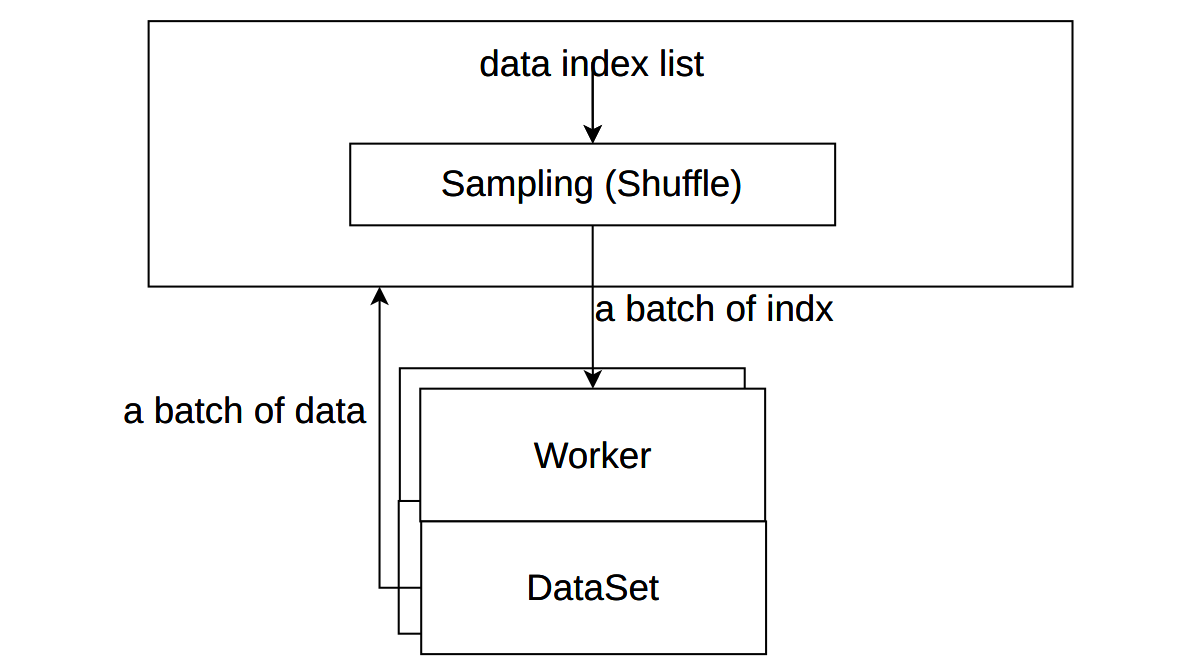
\includegraphics[height=6cm]{global_img_dir/2021-03-02_15-33.png}
    \end{center}
\end{frame}

\begin{frame}
    \frametitle{Problem: Repeated Reading and Processing}
    \begin{block}{Situation}
        To compare the performance of different algorithms, Many DeepLearning tasks are training in the same Dataset.
    \end{block}
    \begin{block}{Problem}
        Every task has its own DataLoader. So the data will be repeatedly read and processed by different tasks.
    \end{block}
    \begin{block}{Result}
        As the number of tasks increases, so does the training time. And what increases is the time to load the data
    \end{block}
\end{frame}

\begin{frame}
    \frametitle{Experiment}
    \begin{figure}[htbp]
    \centering
    \begin{minipage}[t]{0.48\textwidth}
    \centering
    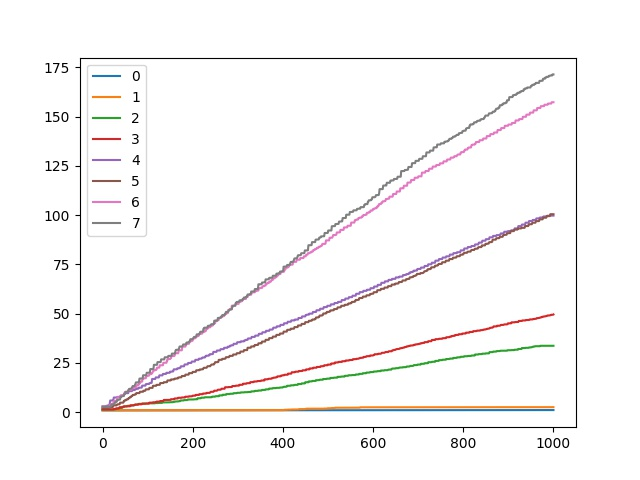
\includegraphics[width=6cm]{global_img_dir/l.jpg}
    \caption{data loading time}
    \end{minipage}
    \begin{minipage}[t]{0.48\textwidth}
    \centering
    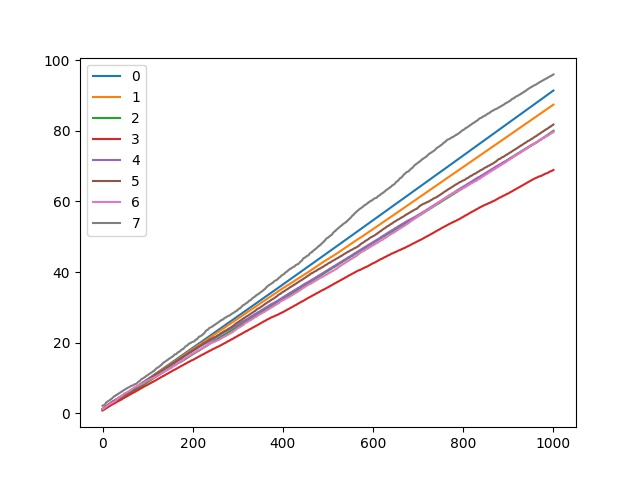
\includegraphics[width=6cm]{global_img_dir/b.jpg}
    \caption{data training time}
    \end{minipage}
    \end{figure}
\end{frame}

\section{Global DataLoader}
\begin{frame}
    \frametitle{Architecture}
    \centering
    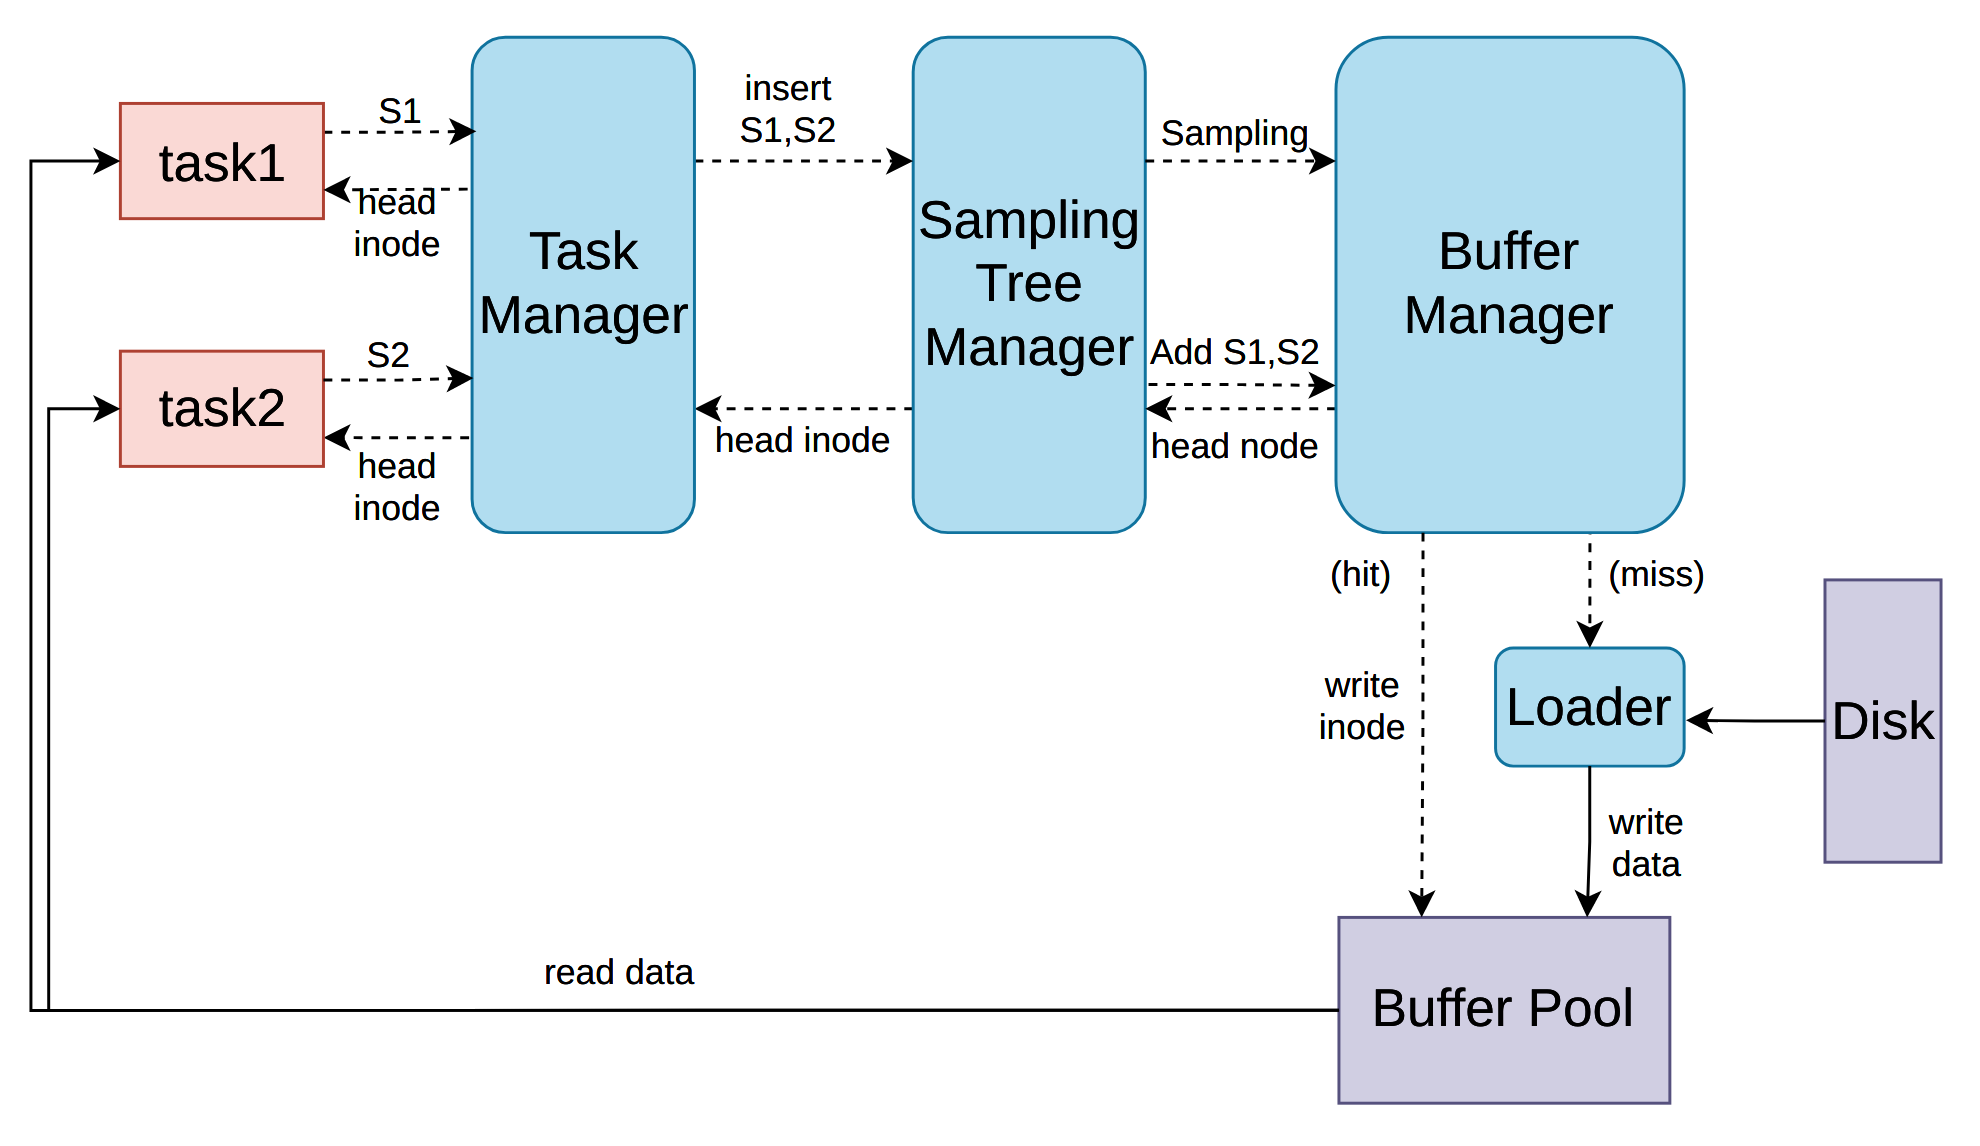
\includegraphics[width=12cm]{global_img_dir/archi.png}
\end{frame}

\begin{frame}
    \frametitle{Sampling: problem description}
    \begin{block}{Defination}
        For a single task, the sampler needs to select an index from the index set $S$.\\
        Similarly, for multiple tasks, the sampler needs to select an index from multiple sets $\{S_1, S_2, ...\}$
    \end{block}
    \begin{block}{Requirments}
        \begin{itemize}
            \item The index in the set $S$ should be randomly sampled. The probability of the index being selected is $1/|S|$
            \item Duplicate indexes need to be merged
            \item There can be no problem of "starvation"
        \end{itemize}
    \end{block}
\end{frame}

\begin{frame}
    \frametitle{Assumption 1}
    \begin{block}{Requirments}
        \begin{itemize}
            \item There are only two sets $\{S_1, S_2\}$
            \item $S_1$ is same as $S_2$. And the length of $S_1$ and $S_2$ is n
        \end{itemize}
    \end{block}
\end{frame}

\begin{frame}
    \frametitle{Solution 1}
    \begin{block}{description}
        In order to avoid the problem of "starvation", we sampling the idx through polling. 
    \end{block}
    \begin{block}{steps}
        \begin{itemize}
            \item First, We randomly select an idx $i_1$ from the $S_1$.
            \item Because $S_1$ and $S_2$ are the same, we don't need to sample $S_2$
        \end{itemize}
    \end{block}
\end{frame}

\begin{frame}
    \frametitle{Assumption 2}
    \begin{block}{Requirments}
        \begin{itemize}
            \item There are only two sets $\{S_1, S_2\}$
            \item $S_1$ and $S_2$ are equal in length, which is $n$
            \item The intersection of $S_1$ and $S_2$ is $S_i$, whose length is $n_i$
        \end{itemize}
    \end{block}
\end{frame}
\begin{frame}
    \frametitle{Solution 2}
    \begin{block}{steps}
        \begin{itemize}
            \item First, We randomly select an idx $i_1$ from the $S_1$.
            \item If $i_1 \in S_2$, then we do nothing like solution 1
            \item If $i_1 \notin S_2$, then we randomly select an idx $i_2$ from the $S_2-S_1$
        \end{itemize}
    \end{block}
\end{frame}
\begin{frame}
    \frametitle{Proving}
    \begin{block}{S1}
        $p(idx_1) = \frac{1}{n}$
    \end{block}
    \begin{block}{S2}
        If $idx_2 \in S_i$, 
        $$
            p(idx_2) = \frac{n_i}{n}*\frac{1}{n_i} = \frac{1}{n}
        $$
        If $idx_2 \notin S_i$, 
        $$
            p(idx_2) = \frac{n-n_i}{n}*\frac{1}{n-n_i} = \frac{1}{n}
        $$
    \end{block}
\end{frame}

\begin{frame}
    \frametitle{Assumption 3}
    \begin{block}{Requirments}
        \begin{itemize}
            \item There are only two sets $\{S_1, S_2\}$
            \item $S_1$ is different from $S_2$, and their length are $n_1$ and $n_2$
            \item The intersection of $S_1$ and $S_2$ is $S_i$, whose length is $n_i$
        \end{itemize}
    \end{block}
\end{frame}

\begin{frame}
    \frametitle{Solution 3}
    If we use Solution2.
    \begin{block}{S2}
        If $idx_2 \in S_i$, 
        $$
            p(idx_2) = \frac{n_i}{n_1}*\frac{1}{n_i} = \frac{1}{n_1}
        $$
        If $idx_2 \notin S_i$, 
        $$
            p(idx_2) = \frac{n_1-n_i}{n_1}*\frac{1}{n2-n_i} = \frac{n_1-n_i}{n_1*(n_2-n_i)}
        $$
    \end{block}
\end{frame}

\begin{frame}
    \frametitle{Solution 3}
        if $n_1 < n_2$, then $p(idx_2 \in S_i) > \frac{1}{n_2}$. So in step 2 of Solution2, we should randomly select a idx in $S_2-S_i$ in probability of $x$.\\
        \begin{block}
        If $idx_2 \in S_i$, 
        $$
            p(idx_2) = \frac{n_i}{n_1}*(1-x)*\frac{1}{n_i} = \frac{1}{n_2}
        $$
        If $idx_2 \notin S_i$, 
        $$
            p(idx_2') = \frac{n_1-n_i}{n_1}*\frac{1}{n2-n_i} + \frac{n_i}{n_1}*x*\frac{1}{n2-n_i} = \frac{1}{n_2}
        $$
        then
        $$
            x = \frac{n_2-n_1}{n_2}
        $$
    \end{block}
\end{frame}

\begin{frame}
    \frametitle{Solution 3}
        if $n_1 > n_2$, then $p(idx_2 \notin S_i) > \frac{1}{n_2}$. So in step 3 of Solution2, we should randomly select a idx in $S_i$ in probability of $x$.\\
        \begin{block}
        If $idx_2 \in S_i$, 
        $$
            p(idx_2) = \frac{n_i}{n_1}*\frac{1}{n_i}+x*\frac{n1-n_c}{n1}*\frac{1}{n_i} = \frac{1}{n_2}
        $$
        If $idx_2 \notin S_i$, 
        $$
        \frac{n1-n_i}{n1}*\frac{1}{(n2-n_i)}*(1-x) = \frac{1}{n2}
        $$
        then
        $$
            x = 1-\frac{n_1*(n_2-n_i)}{n_2*(n_1-n_i)}
        $$
    \end{block}
\end{frame}

\begin{frame}
    \frametitle{Solution 3}
        \begin{block} {steps}
            \begin{itemize}
                \item First, We randomly select an idx $i_1$ from the $S_1$.
                \item If $i_1 \in S_2$ and $n_1 < n_2$, randomly sample in $S_2-S_i$ with a probability of $\frac{n_2-n_1}{n_2}$ 
                \item If $i_1 \in S_2$ and $n_1 > n_2$, do nothing
                \item If $i_1 \notin S_2$ and $n_1 > n_2$, randomly sample in $S_2-S_i$ with a probability of $1-\frac{n_1*(n_2-n_i)}{n_2*(n_1-n_i)}$
                \item If $i_1 \notin S_2$ and $n_1 < n_2$, do nothing
            \end{itemize}
        \end{block}
\end{frame}

\begin{frame}[fragile]
    \frametitle{Data Structure}
    \begin{lstlisting}
        
    \end{lstlisting}
\end{frame}

\begin{frame}[fragile]
    \frametitle{Insert}
    \begin{lstlisting}
        
    \end{lstlisting}
\end{frame}

\begin{frame}[fragile]
    \frametitle{Sample}
    \begin{lstlisting}
        
    \end{lstlisting}
\end{frame}

\begin{frame}
    \frametitle{Buffer Pool: Data Structure}
    \centering
    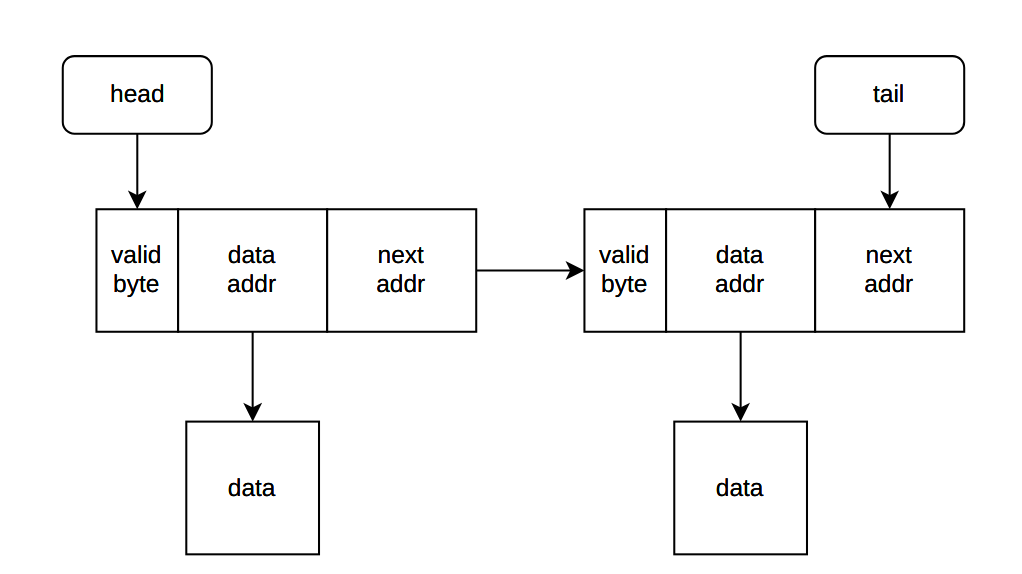
\includegraphics[width=10cm]{global_img_dir/linklist.png}
\end{frame}

\begin{frame}
    \frametitle{Buffer Pool: Valid Byte}
    \begin{block} {valid byte}
        \begin{itemize}
            \item data bit: If the data bit is equal to 1, the data addr is valid. Otherwise invalid
            \item next bit: If the next bit is equal to 1, the next addr is valid. Otherwise invalid
            \item used bit: If the used bit is equal to 1, this inode is used by some tasks
        \end{itemize}
    \end{block}
\end{frame}

\begin{frame}
    \frametitle{Buffer Pool: Automata}
    \centering
    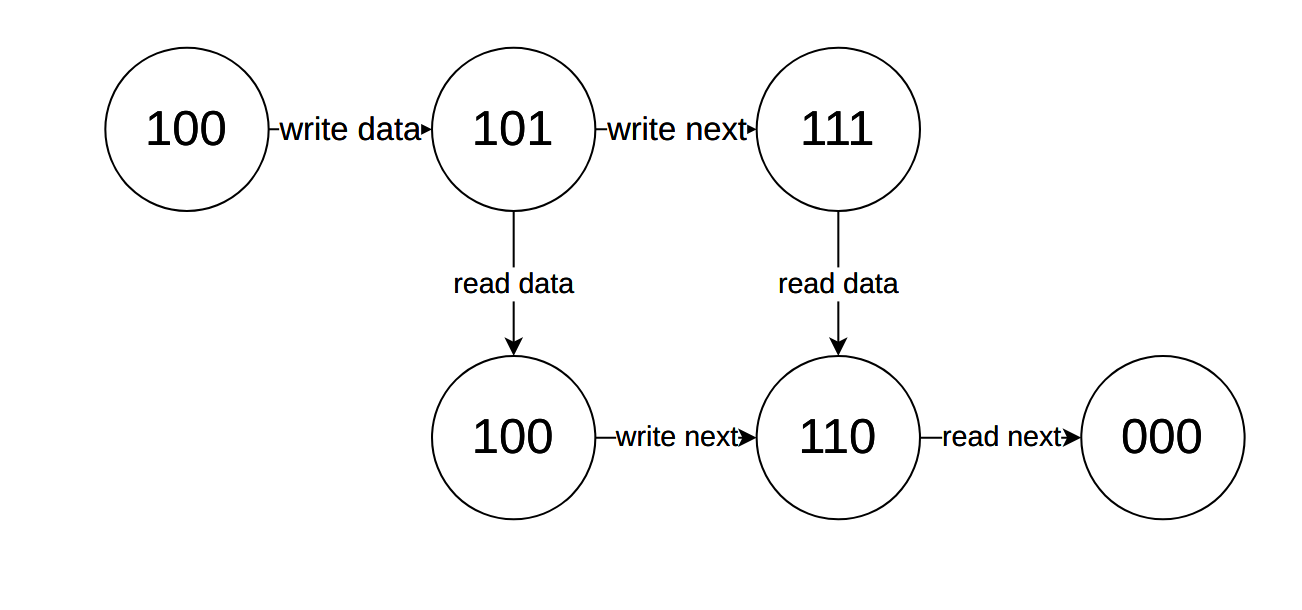
\includegraphics[width=12cm]{global_img_dir/automata.png}
\end{frame}

\begin{frame}
    \frametitle{Buffer Pool: Address Space}
    \centering
    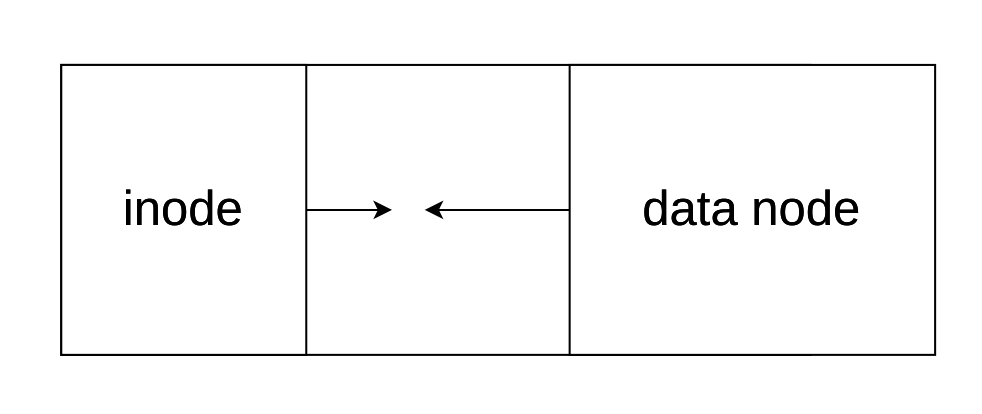
\includegraphics[width=12cm]{global_img_dir/space.png}
\end{frame}

\begin{frame}
    \frametitle{Buffer Pool: allocate inode}
\end{frame}

\begin{frame}
    \frametitle{Buffer Pool: allocate data node}
\end{frame}

\begin{frame}
    \frametitle{Buffer Pool: write}
\end{frame}

\begin{frame}
    \frametitle{Buffer Pool: read}
\end{frame}
\section{Experiment}

\begin{frame}
    \frametitle{Experiment}
    \begin{figure}[htbp]
        \centering
        \begin{minipage}[t]{0.48\textwidth}
        \centering
        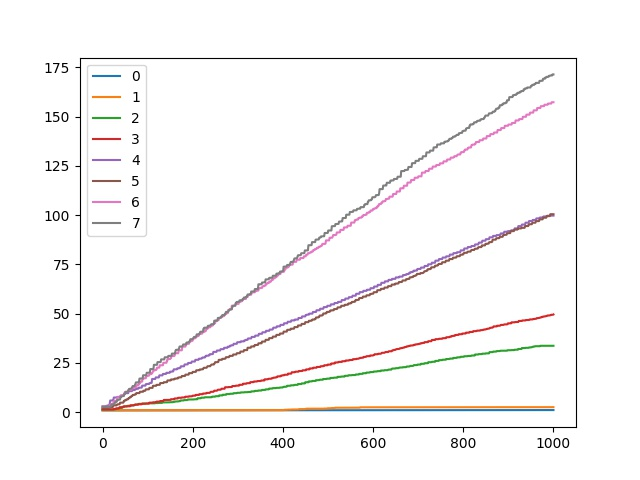
\includegraphics[width=6cm]{global_img_dir/l.jpg}
        \caption{time}
        \end{minipage}
        \begin{minipage}[t]{0.48\textwidth}
        \centering
        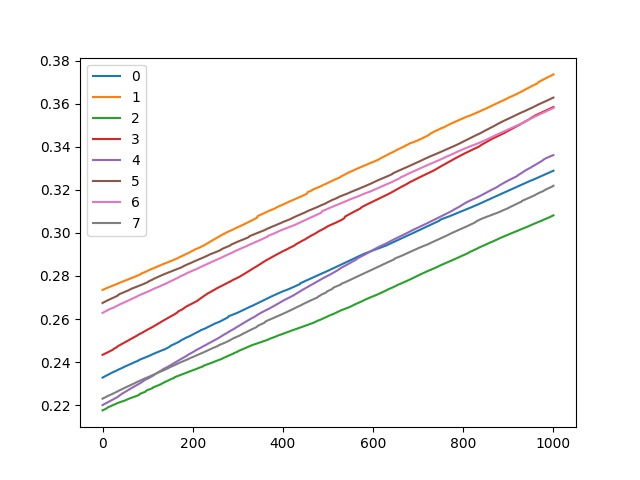
\includegraphics[width=6cm]{global_img_dir/gl.jpg}
        \caption{time with GlobalDataLoader}
        \end{minipage}
    \end{figure}
\end{frame}

\end{document}